\renewcommand{\thefigure}{8.\arabic{figure}}
\section*{Глава 8. Взаимное вытеснение жидкостей и газов. Задачи с подвижными границами}
% Источник: Basniev-et-al.djvu; печатная страница: 188; страница файла: 189
\subsection*{§ 1. Кинематические условия на подвижной границе раздела при взаимном вытеснении жидкостей}
Основная трудность точного решения задачи о движении границы раздела двух жидкостей в пористой среде заключается в том, что линии тока на границе раздела жидкостей преломляются.

Пусть кривая $I$--$I$ (рис. \ref{q9:fig-8-1}) является границей раздела двух жидкостей с вязкостями $\mu_1$ и $\mu_2$ и пусть, например, $\mu_2>\mu_1$ (нефть вытесняется водой). Рассмотрим произвольную точку $M$ границы $I$--$I$ и проведем через нее касательную $\vec\tau$ и нормаль $\vec n$ к границе раздела жидкостей $I$--$I$. Найдем проекции скоростей фильтрации воды и нефти, находящихся в данный момент в точке $M$, на касательную $\vec\tau$ и нормаль $\vec n$, считая проницаемость пористой среды $k$ постоянной по обе стороны границы раздела.
\begin{figure}[H]\centering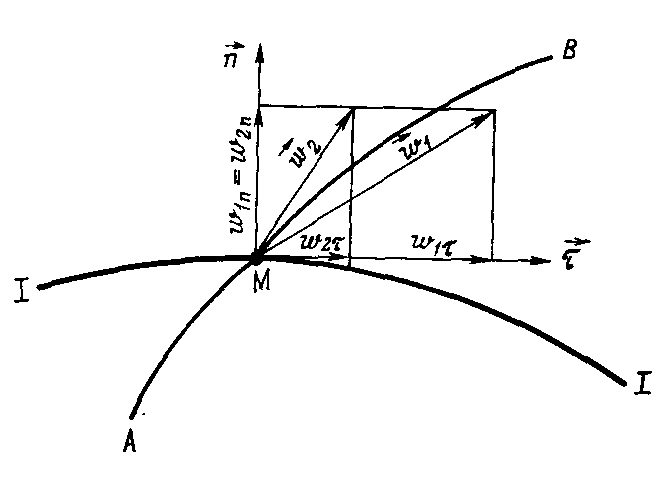
\includegraphics[width=.65\linewidth]{figures/fig-8-1.png}\caption{Преломление линий тока на границе раздела жидкостей}\label{q9:fig-8-1}\end{figure}
Согласно условию неразрывности потока массы элементарные расходы обеих несжимаемых жидкостей через элемент границы раздела, включающий точку $M$, должны быть равны между собой. Отсюда следует, что нормальные составляющие скоростей фильтрации обеих жидкостей будут равны, т. е. $w_{1n}=w_{2n}$. Давление в пласте в точке $M$ также должно быть одинаково для обеих жидкостей, так как при малых скоростях (ниже звуковых) разрыва давления в сплошном потоке быть не может. Касательные составляющие скоростей фильтрации обеих жидкостей будут определяться по закону Дарси:
\begin{equation}w_{1\tau}=-\frac{k}{\mu_1}\frac{\partial p}{\partial\tau};\tag{8.1}\label{q9:eq-8-1}\end{equation}
\begin{equation}w_{2\tau}=-\frac{k}{\mu_2}\frac{\partial p}{\partial\tau}.\tag{8.2}\label{q9:eq-8-2}\end{equation}
Так как $\mu_2>\mu_1$, то из \eqref{q9:eq-8-1} и \eqref{q9:eq-8-2} получаем, что $w_{1\tau}>w_{2\tau}$. Отсюда следует, что результирующий вектор скорости фильтрации $\vec w_1$ ($\vec w_1=\vec w_{1\tau}+\vec w_{1n}$), касательный к линии тока $AM$, будет больше вектора $\vec w_2$ ($\vec w_2=\vec w_{2\tau}+\vec w_{2n}$), касательного к линии тока нефти $MB$. Следовательно, линии тока $AM$ и $MB$, проходящие
% Источник: Basniev-et-al.djvu; печатная страница: 189; страница файла: 190
через точку $M$, будут иметь излом в точке $M$. Учет этого преломления линий тока на границе раздела жидкостей и составляет главную трудность в точном решении задачи продвижения границы раздела.

Линии тока не будут преломляться только в двух случаях --- при прямолинейно-параллельном и плоскорадиальном движениях границы раздела, когда $w_{1\tau}=w_{2\tau}=0$. Эти задачи прежде всего и будут рассмотрены в данной главе. При этом жидкости (нефть и вода) считаются несжимаемыми, взаимно нерастворимыми и химически не реагирующими одна с другой и с пористой средой. Вытеснение нефти водой предполагается происходящим полностью --- так называемое поршневое вытеснение. Задачи, в которых учитывается неполнота вытеснения, рассматриваются в гл. 9.

\subsection*{§ 2. Прямолинейно-параллельное вытеснение нефти водой}
При поршневом вытеснении нефти водой в пористой среде плотности нефти и воды будем считать одинаковыми. Это позволит рассматривать плоскость контакта нефти и воды вертикальной. А различие в вязкостях нефти $\mu_\text{н}$ и воды $\mu_\text{в}$ будем учитывать.

В случае прямолинейно-параллельного движения схема вытеснения представлена на рис. \ref{q9:fig-8-2}. На контуре питания и на галерее поддерживаются соответственно постоянные давления $p_\text{к}$ и $p_\text{г}$. Начальное положение контура нефтеносности $x_0$ параллельно галерее и контуру питания.
\begin{figure}[H]\centering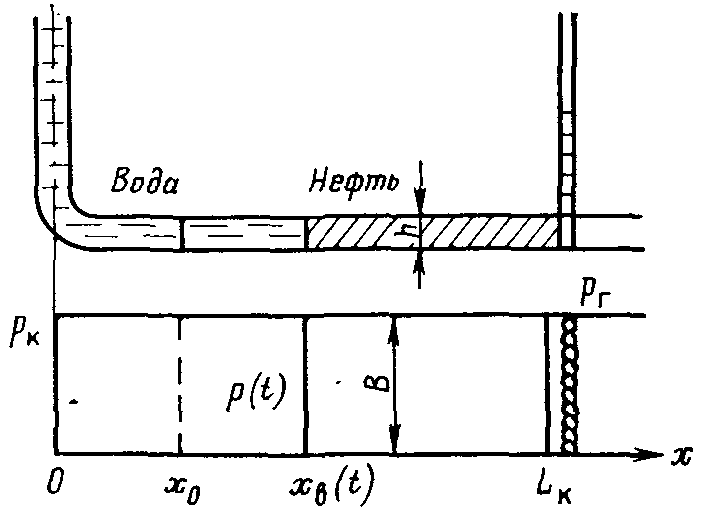
\includegraphics[width=.78\linewidth]{figures/fig-8-2.png}\caption{Схема модели пласта при прямолинейно-параллельном движении границы раздела вода---нефть}\label{q9:fig-8-2}\end{figure}
Обозначим через $x_\text{в}$ текущее расстояние до контура нефтеносности в момент времени $t$ после начала вытеснения, через $L_\text{к}$ --- расстояние от контура питания до галереи, через $p_\text{в},p_\text{н}$ --- давление в любой точке водоносной и нефтеносной части пласта соответственно, через $p(t)$ --- давление на границе раздела вода---нефть, отстоящей от контура питания на расстоянии $x_\text{в}$.

Вспомним, что в случае установившегося прямолинейно-параллельного фильтрационного потока одной жидкости (см. § 2 гл. 4) распределение давления и скорость фильтрации описываются следующими уравнениями:
\begin{equation}p=p_\text{к}-\frac{p_\text{к}-p_\text{г}}{L_\text{к}}x=p_\text{г}+\frac{p_\text{к}-p_\text{г}}{L_\text{к}}(L_\text{к}-x);\tag{8.3}\label{q9:eq-8-3}\end{equation}
\begin{equation}w=\frac{k}{\mu}\frac{p_\text{к}-p_\text{г}}{L_\text{к}}.\tag{8.4}\label{q9:eq-8-4}\end{equation}
% Источник: Basniev-et-al.djvu; печатная страница: 190; страница файла: 191
При этом изобарами являются линии, параллельные галерее, и каждую изобару можно рассматривать как контур питания или как галерею. На основании формул \eqref{q9:eq-8-3} и \eqref{q9:eq-8-4} распределение давления и скорость фильтрации в водоносной области можно записать в виде
\begin{equation}p_\text{в}=p_\text{к}-\frac{p_\text{к}-p(t)}{x_\text{в}(t)}x,\quad0\le x\le x_\text{в}(t);\tag{8.5}\label{q9:eq-8-5}\end{equation}
\begin{equation}w_\text{в}=\frac{k}{\mu_\text{в}}\frac{p_\text{к}-p(t)}{x_\text{в}(t)}.\tag{8.6}\label{q9:eq-8-6}\end{equation}
Принимая за контур питания изобару, совпадающую с границей раздела жидкостей, распределение давления и скорость фильтрации в нефтеносной области можно записать следующим образом:
\begin{equation}p_\text{н}=p_\text{г}+\frac{p(t)-p_\text{г}}{L_\text{к}-x_\text{в}(t)}(L_\text{к}-x),\quad x_\text{в}(t)\le x\le L_\text{к};\tag{8.7}\label{q9:eq-8-7}\end{equation}
\begin{equation}w_\text{н}=\frac{k}{\mu_\text{н}}\frac{p(t)-p_\text{г}}{L_\text{к}-x_\text{в}(t)}.\tag{8.8}\label{q9:eq-8-8}\end{equation}
Найдем давление $p(t)$ на границе раздела. Вследствие несжимаемости жидкостей и неразрывности потока линии тока будут иметь вид прямых, параллельных оси $Ox$ (на границе раздела преломления не будет), а скорость фильтрации во всех точках пласта будет одинаковой, т. е. $w_\text{в}=w_\text{н}$.

Тогда из уравнений \eqref{q9:eq-8-6} и \eqref{q9:eq-8-8} получим
\begin{equation}\frac{k(p_\text{к}-p(t))}{\mu_\text{в}x_\text{в}(t)}=\frac{k(p(t)-p_\text{г})}{\mu_\text{н}(L_\text{к}-x_\text{в}(t))},\tag{8.9}\label{q9:eq-8-9}\end{equation}
откуда давление на границе раздела жидкостей будет
\begin{equation}p(t)=\frac{p_\text{к}\mu_\text{н}(L_\text{к}-x_\text{в}(t))+p_\text{г}\mu_\text{в}x_\text{в}(t)}{\mu_\text{в}x_\text{в}(t)+\mu_\text{н}(L_\text{к}-x_\text{в}(t))}.\tag{8.10}\label{q9:eq-8-10}\end{equation}
Определим теперь следующие характеристики фильтрационного потока нефти и воды.

1. Распределение давления в водоносной и нефтеносной областях. Для этого подставим \eqref{q9:eq-8-10} в \eqref{q9:eq-8-5} и \eqref{q9:eq-8-7}:
\begin{equation}p_{(\text{в})}=p_\text{к}-\frac{\mu_\text{в}(p_\text{к}-p_\text{г})}{\mu_\text{в}x_\text{в}(t)+\mu_\text{н}(L_\text{к}-x_\text{в}(t))}x;\tag{8.11}\label{q9:eq-8-11}\end{equation}
\begin{equation}p_{(\text{н})}=p_\text{г}+\frac{\mu_\text{н}(p_\text{к}-p_\text{г})}{\mu_\text{в}x_\text{в}(t)+\mu_\text{н}(L_\text{к}-x_\text{в}(t))}(L_\text{к}-x).\tag{8.12}\label{q9:eq-8-12}\end{equation}
2. Скорость фильтрации. Подставим \eqref{q9:eq-8-10} в \eqref{q9:eq-8-6} и \eqref{q9:eq-8-8}:
\begin{equation}w_\text{в}=w_\text{н}=\frac{k(p_\text{к}-p_\text{г})}{\mu_\text{в}x_\text{в}(t)+\mu_\text{н}(L_\text{к}-x_\text{в}(t))}.\tag{8.13}\label{q9:eq-8-13}\end{equation}
3. Расход жидкости (дебит галереи) $Q$.
% Источник: Basniev-et-al.djvu; печатная страница: 191; страница файла: 192
Умножим \eqref{q9:eq-8-13} на площадь сечения потока $Bh$:
\begin{equation}Q=\frac{k(p_\text{к}-p_\text{г})}{\mu_\text{в}x_\text{в}(t)+\mu_\text{н}(L_\text{к}-x_\text{в}(t))}Bh.\tag{8.14}\label{q9:eq-8-14}\end{equation}
1. Градиент давления. Продифференцируем \eqref{q9:eq-8-11} и \eqref{q9:eq-8-12} по $x$:
% В оригинале пункт имеет номер 1, а следующий пункт — 5; сохранено.
\begin{equation}\frac{\partial p_{(\text{в})}}{\partial x}=-\frac{\mu_\text{в}(p_\text{к}-p_\text{г})}{\mu_\text{в}x_\text{в}(t)+\mu_\text{н}(L_\text{к}-x_\text{в}(t))};\tag{8.15}\label{q9:eq-8-15}\end{equation}
\begin{equation}\frac{\partial p_{(\text{н})}}{\partial x}=-\frac{\mu_\text{н}(p_\text{к}-p_\text{г})}{\mu_\text{в}x_\text{в}(t)+\mu_\text{н}(L_\text{к}-x_\text{в}(t))}.\tag{8.16}\label{q9:eq-8-16}\end{equation}
5. Закон движения границы раздела $x_\text{в}=x_\text{в}(t)$ находим из соотношения скорости фильтрации и средней скорости движения:
\[w=mv=m\frac{dx_\text{в}}{dt},\]
откуда
\begin{equation}dt=\frac{m}{w}dx_\text{в}=\frac{m}{\dfrac{k(p_\text{к}-p_\text{г})}{\mu_\text{в}x_\text{в}(t)+\mu_\text{н}(L_\text{к}-x_\text{в}(t))}}dx_\text{в}.\tag{8.17}\label{q9:eq-8-17}\end{equation}
Проинтегрировав \eqref{q9:eq-8-17} в пределах от 0 до $t$ и от $x_0$ до $x_\text{в}$, получим
\begin{equation}t=\frac{m}{k(p_\text{к}-p_\text{г})}\left[\mu_\text{н}L_\text{к}(x_\text{в}-x_0)-\frac12(\mu_\text{н}-\mu_\text{в})(x_\text{в}^2-x_0^2)\right].\tag{8.18}\label{q9:eq-8-18}\end{equation}
Чтобы найти время полного вытеснения нефти, нужно в формуле \eqref{q9:eq-8-18} положить $x_\text{в}=L_\text{к}$. Тогда получим
\[T=\frac{m}{2k(p_\text{к}-p_\text{г})}\left[\mu_\text{в}(L_\text{к}^2-x_0^2)+\mu_\text{н}(L_\text{к}-x_0)^2\right].\]
Для нахождения зависимости координаты границы раздела $x_\text{в}$ от времени $t$ решим квадратное уравнение \eqref{q9:eq-8-18} относительно $x_\text{в}$:
\begin{equation}x_\text{в}=\frac{\mu_\text{н}}{\mu_\text{н}-\mu_\text{в}}L_\text{к}-\sqrt{\left(\frac{\mu_\text{н}}{\mu_\text{н}-\mu_\text{в}}L_\text{к}-x_0\right)^2+\frac{2k(p_\text{к}-p_\text{г})}{m(\mu_\text{н}-\mu_\text{в})}t}.\tag{8.19}\label{q9:eq-8-19}\end{equation}
% В (8.19) знак + перед членом с t напечатан в оригинале; не исправлен.
Подставив это значение $x_\text{в}$ в формулы \eqref{q9:eq-8-13} и \eqref{q9:eq-8-14}, найдем изменение скорости фильтрации и дебита галереи во времени:
\begin{equation}w=\frac{k(p_\text{к}-p_\text{г})}{\sqrt{[\mu_\text{н}L_\text{к}-(\mu_\text{н}-\mu_\text{в})x_0]^2-\dfrac{2k(p_\text{к}-p_\text{г})}{m}(\mu_\text{н}-\mu_\text{в})t}};\tag{8.20}\label{q9:eq-8-20}\end{equation}
\begin{equation}Q=\frac{kBh(p_\text{к}-p_\text{г})}{\sqrt{[\mu_\text{н}L_\text{к}-(\mu_\text{н}-\mu_\text{в})x_0]^2-\dfrac{2k(p_\text{к}-p_\text{г})}{m}(\mu_\text{н}-\mu_\text{в})t}}.\tag{8.21}\label{q9:eq-8-21}\end{equation}
Проанализируем полученные характеристики потока.

1. Из уравнений \eqref{q9:eq-8-11} и \eqref{q9:eq-8-12} видно, что давление в пласте зависит не только от координаты $x$, но и от положения границы
% Источник: Basniev-et-al.djvu; печатная страница: 192; страница файла: 193
раздела $x_\text{в}$. Но $x_\text{в}$, как это следует из формулы \eqref{q9:eq-8-19}, со временем увеличивается, следовательно, пластовое давление во времени в водоносной области падает, а в нефтеносной --- растет. На рис. \ref{q9:fig-8-3} показано распределение давления в пласте в начальный момент вытеснения, когда граница раздела занимает положение $x_0$, и некоторое время $t$ спустя, когда граница раздела продвинулась до положения $x_\text{в}$. Из графика видно, что пьезометрическая линия на границе раздела имеет излом.
\begin{figure}[H]\centering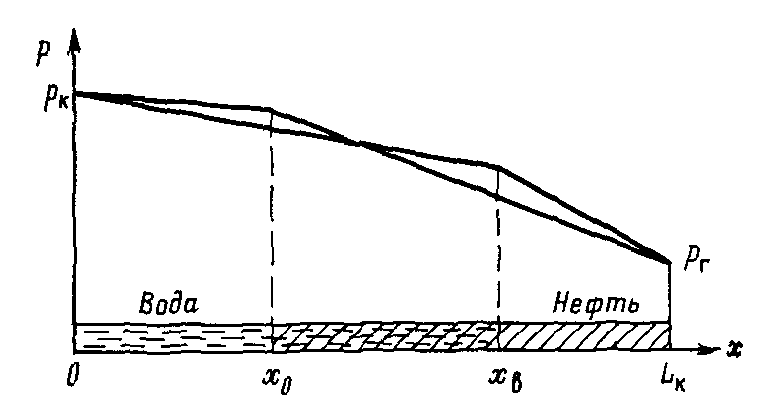
\includegraphics[width=.75\linewidth]{figures/fig-8-3.png}\caption{Кривые распределения давления в пласте при вытеснении нефти водой}\label{q9:fig-8-3}\end{figure}
2. Скорость фильтрации $w$ \eqref{q9:eq-8-20} и расход жидкости $Q$ \eqref{q9:eq-8-21} также изменяются во времени. Следовательно, несмотря на постоянство депрессии $\Delta p=p_\text{к}-p_\text{г}$ движение жидкостей в пласте будет неустановившимся.

При $\mu_\text{н}>\mu_\text{в}$, как видно из указанных формул, скорость фильтрации и дебит галереи увеличиваются с течением времени, т. е. по мере продвижения контура нефтеносности.

Это легко объяснимо и из физических соображений. Движение жидкостей в пласте происходит под действием постоянного перепада давления $\Delta p$. Величина же сопротивления, оказываемого обеими жидкостями, зависит от размеров их областей. С течением времени увеличивается область водоносности, сопротивление которой по сравнению с областью нефтеносности тех же размеров значительно меньше. Следовательно, общее сопротивление обеих областей во времени уменьшается, что при постоянной депрессии $\Delta p$ ведет к росту скорости фильтрации и дебита галереи.

3. Градиенты давления в водоносной и нефтеносной областях, как это следует из формул \eqref{q9:eq-8-15} и \eqref{q9:eq-8-16} с учетом \eqref{q9:eq-8-19}, увеличиваются во времени. Это же видно и из рис. \ref{q9:fig-8-3}. В нефтеносной области градиент давления больше, чем в водоносной во столько раз, во сколько вязкость нефти больше вязкости воды.

Если первоначальное положение водонефтяного контакта $AB$ в пласте не параллельно галерее (рис. \ref{q9:fig-8-4}), то решить задачу можно только приближенно, например используя метод «полосок», предложенный В. Н. Щелкачевым. В потоке выделяются узкие полоски,
\begin{figure}[H]\centering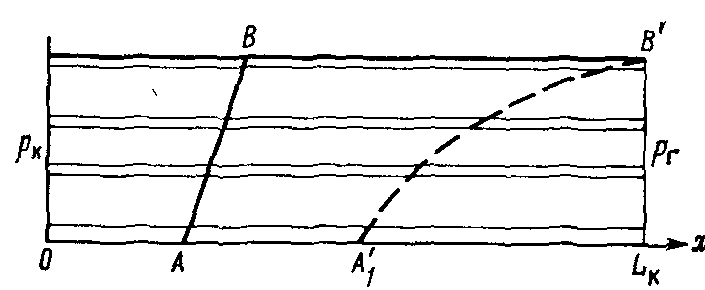
\includegraphics[width=.8\linewidth]{figures/fig-8-4.png}\caption{Схема использования метода «полосок»}\label{q9:fig-8-4}\end{figure}
% Источник: Basniev-et-al.djvu; печатная страница: 193; страница файла: 194
в пределах каждой из которых водонефтяной контакт считается параллельным галерее, и движение в каждой полоске описывается выведенными в этом параграфе формулами. При этом, как видно из формулы \eqref{q9:eq-8-20}, чем больше $x_0$, тем больше скорость фильтрации $w$. Отсюда вытекает, что граница раздела в точке $B$ будет двигаться гораздо быстрее, чем в точке $A$, и обводнение галереи начнется именно по линии $BB'$, в то время как контур нефтеносности по другим линиям будет еще значительно удален от галереи. Из этого примера следует важное заключение о характере продвижения контура нефтеносности. Если на границе раздела вода---нефть при разработке нефтяной залежи образовался «водяной язык», то он в дальнейшем не только не исчезает, а быстро вытягивается, продвигаясь с большей скоростью, чем остальная часть водонефтяного контакта.

% Источник: Basniev-et-al.djvu; печатная страница: 196; страница файла: 197
\subsection*{§ 4. Устойчивость движения границы раздела жидкостей}
В реальных условиях движение границы раздела жидкостей, естественно, сложнее, чем по рассмотренным выше схемам, так как водонефтяной (газоводяной) контакт совершает сложное пространственное движение. В реальных условиях продуктивные пласты наклонны и граница раздела жидкостей, имеющая горизонтальное начальное положение, в процессе разработки залежи нефти (газа) деформируется.

% Источник: Basniev-et-al.djvu; печатная страница: 197; страница файла: 198
Пусть нефтяная залежь в наклонном пласте (рис. \ref{q9:fig-8-6}) имеет горизонтальное начальное положение водонефтяного контакта $A_0B_0$.

При отборе нефти граница раздела вода---нефть будет перемещаться, занимая последовательно положения $A_1B_1$, $A_2B_2$ и т. д. Рассмотрим вопрос об устойчивости движения границы раздела. Скорости фильтрации каждой жидкости согласно закону Дарси определяются при учете силы тяжести по формулам
\begin{equation}\begin{aligned}
w_\text{в}&=-\frac{k_1}{\mu_\text{в}}\left(\frac{\partial p}{\partial s}+\rho_\text{в}g\frac{\partial z}{\partial s}\right);&w_\text{н}&=-\frac{k_2}{\mu_\text{н}}\left(\frac{\partial p}{\partial s}+\rho_\text{н}g\frac{\partial z}{\partial s}\right).
\end{aligned}\tag{8.39}\label{q9:eq-8-39}\end{equation}
Вследствие неизбежных возмущений на границе раздела частицы воды попадают в область, занятую нефтью, при этом их дальнейшее движение может либо ускоряться, либо замедляться. В первом случае, при ускорении движения частиц воды, движение границы раздела будет неустойчивым; во втором, при замедлении движения частиц воды, --- устойчивым.
\renewcommand{\thefigure}{8.\arabic{figure}}\setcounter{figure}{5}
\begin{figure}[H]\centering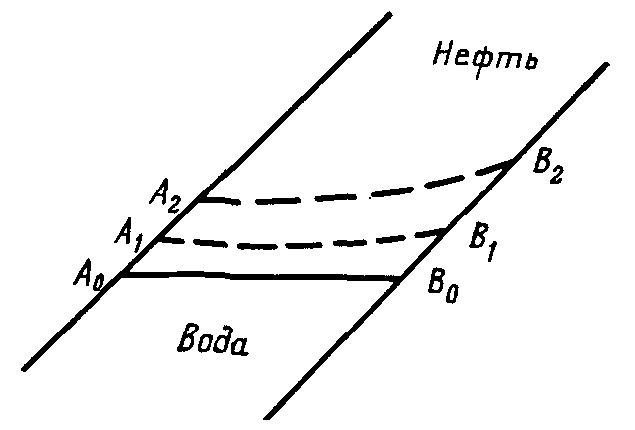
\includegraphics[width=.7\linewidth]{figures/fig-8-6.png}\caption{Схема движения водонефтяного контакта в наклонном пласте}\label{q9:fig-8-6}\end{figure}
Условия устойчивости движения границы раздела можно установить из следующих элементарных соображений. Обозначим через $(w_\text{в})_\text{н}$ скорость фильтрации частиц воды, попавших в поток нефти с градиентом давления $(\partial p/\partial s)_\text{н}$; через $(k_1)_2$ --- проницаемость пласта для воды в зоне движения нефти.

Тогда из первого соотношения \eqref{q9:eq-8-39} имеем
\begin{equation}(w_\text{в})_\text{н}=-\frac{(k_1)_2}{\mu_\text{в}}\left[\left(\frac{\partial p}{\partial s}\right)_\text{н}+\rho_\text{в}g\frac{\partial z}{\partial s}\right].\tag{8.40}\label{q9:eq-8-40}\end{equation}
Скорость фильтрации основных частиц нефти, соприкасающихся с проникшими туда частицами воды, согласно второму уравнению \eqref{q9:eq-8-39} будет
\begin{equation}w_\text{н}=-\frac{k_2}{\mu_\text{н}}\left[\left(\frac{\partial p}{\partial s}\right)_\text{н}+\rho_\text{н}g\frac{\partial z}{\partial s}\right].\tag{8.41}\label{q9:eq-8-41}\end{equation}
Из уравнений \eqref{q9:eq-8-40} и \eqref{q9:eq-8-41} получаем связь между скоростями фильтрации $(w_\text{в})_\text{н}$ и $w_\text{н}$:
\[
\frac{\mu_\text{в}}{(k_1)_2}(w_\text{в})_\text{н}+\rho_\text{в}g\frac{\partial z}{\partial s}=\frac{\mu_\text{н}}{k_2}w_\text{н}+\rho_\text{н}g\frac{\partial z}{\partial s}=-\left(\frac{\partial p}{\partial s}\right)_\text{н},
\]
откуда
\[
(w_\text{в})_\text{н}=\frac{\mu_\text{н}}{\mu_\text{в}}\frac{(k_1)_2}{k_2}w_\text{н}-\frac{(k_1)_2}{\mu_\text{в}}(\rho_\text{в}-\rho_\text{н})g\frac{\partial z}{\partial s}.
\]
% Источник: Basniev-et-al.djvu; печатная страница: 198; страница файла: 199
Об устойчивости движения границы раздела можно судить по разности скоростей фильтрации:
\begin{equation}\begin{aligned}
\Delta w&=(w_\text{в})_\text{н}-w_\text{н}=\left[\frac{\mu_\text{н}}{\mu_\text{в}}\frac{(k_1)_2}{k_2}-1\right]w_\text{н}-\\
&\quad-\frac{(k_1)_2}{\mu_\text{в}}(\rho_\text{в}-\rho_\text{н})g\frac{\vert\partial z}{\partial s}.
\end{aligned}\tag{8.42}\label{q9:eq-8-42}\end{equation}
% TODO: проверить по оригиналу дополнительный вертикальный штрих перед ∂z в (8.42). На предоставленном скане он виден; сохранён без восстановления по догадке.
При $\Delta w\le0$ движение границы раздела жидкостей будет устойчивым, при $\Delta w\ge0$ движение неустойчиво.

Если угол наклона пласта к горизонту обозначить через $\alpha$, то, очевидно, $\partial z/\partial s=\sin\alpha$.

Тогда условие устойчивости границы раздела \eqref{q9:eq-8-42} можно представить в виде
\[
\Delta w=\left[\frac{\mu_\text{н}}{\mu_\text{в}}\frac{(k_1)_2}{k_2}-1\right]w_\text{н}-\frac{(k_1)_2}{\mu_\text{в}}(\rho_\text{в}-\rho_\text{н})g\sin\alpha.
\]
Обычно $(k_1)_2$ меньше $k_2$. Считая в первом приближении, что $(k_1)_2=k_2$, преобразуем это соотношение к виду
\begin{equation}\Delta w=\left(\frac{\mu_\text{н}}{\mu_\text{в}}-1\right)w_\text{н}-\frac{k_2}{\mu_\text{в}}(\rho_\text{в}-\rho_\text{н})g\sin\alpha.\tag{8.43}\label{q9:eq-8-43}\end{equation}
Так как при устойчивом движении границы раздела $\Delta w\le0$, то из \eqref{q9:eq-8-43} найдем, что при устойчивом движении границы раздела жидкостей скорость фильтрации нефти $w_\text{н}$ на границе раздела должна быть
\[
w_\text{н}\le\frac{k_2}{\mu_\text{н}-\mu_\text{в}}(\rho_\text{в}-\rho_\text{н})g\sin\alpha.
\]
Более строгое исследование рассмотренной задачи проводится методами теории возмущений и гидродинамической устойчивости.
